\chapter{心得}

\section{鍾秉桓 Roy}
\label{sec:Roy}

其實從高中初次接觸程式設計以來,我一直想做的事情便是寫一個自己的遊戲引擎,從高中時初次嘗試撰寫 ADV 類型的遊戲引擎(但受限當時的程式能力,並沒有完成),而到了大學時,
我從很早(大概大二)便找好組員,並且也在系上課程的多個專案中不斷地練習和磨合我們之間的合作,我想做的事便是寫一個屬於自己的遊戲引擎。

從三年級下學期開始,經過了九個月的的開發,坐在電腦前數百小時的奮鬥,我們 RISH 終於將 RishEngine 的功能告一個段落,儘管有些功能是因為專案時程以及目前能力而有缺憾,
但即便如此我們還是完成了這個專案,我們開發了一款 2D 的遊戲引擎,具有 ECS、有引擎編輯器、有 Batch Rendering、有 2D Lighting、有物理引擎、有 Particle System 等。

\begin{figure}[h]
    \begin{center}
    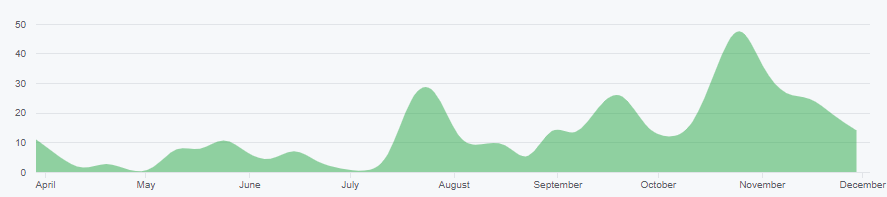
\includegraphics[width=\textwidth]{./resources/ch6/commit.png}
    \end{center}
\caption*{RishEngine Commit Graph}
% \label{fig:RishEngineCommits}
\end{figure}

而在開發每項功能前,都花了一到兩個星期在做資料搜尋、自學,接著做出最小可行的 Demo,僅僅做出功能還不夠,因為我們做得是遊戲引擎,所以還得將 API 打磨,不斷得去想、擴充功能,
因為引擎就是得提供許多功能給遊戲開發者,而在引擎開發階段時,每個功能寫出來之後,還得切換身分到遊戲開發者,試圖用自己做出的引擎來打造遊戲,透過這個過程來除錯和發想可以增加的新功能,
一直不斷的迭代,而這個過程是相當漫長和痛苦的,常常在和組員討論時一個功能的規格(spec)時,往往最後都覺得很迷惘,總是覺得這個功能不夠好,但還是得在現實與理想中取捨。

在這次的專案中我也學到了很多東西,像是如何有效與人溝通和合作,表達自己的想法給對方清楚理解,當然過程中勢必有磨合的時期,因為我們是只有四個人的小組,所以作為組長的我理所當然會處理許多工作,
也必須擔當起管理的責任,畢竟繁雜的工作量由一個人扛起也過於不切實際,清楚了解到除了程式之外管理和與人相處溝通之道也相當重要。

這個畢業專題算是完成了我其中的一個心願,自幹一個遊戲引擎,也是我目前處理過最多行的程式,算是我的一個小小的里程碑。

\section{梁博全 ICEJJ}
\label{sec:ICEJJ}

會開始接觸程式,是因為自己很喜歡玩遊戲,而自己也想開發遊戲,所以想當個遊戲開發者,但隨著深入學習這塊領域,發現市面上遊戲引擎已經很成熟,開發遊戲門檻降低,很多人都能用熱門引擎寫出遊戲。
作為開發者,我們能用現有引擎輕鬆地拉出一款遊戲,我們從中學習到的僅僅只是引擎的使用方法。若未來需要對引擎底層進行優化,但對底層的架構、邏輯都不了解,那要如何修改如何優化。
開發遊戲引擎不只能讓我們更了解遊戲架構,也能更加瞭解一款遊戲的圖形渲染、物理模擬等等是如何運作,我想這會是在眾多遊戲開發者內脫穎而出的關鍵。

在開發引擎功能的,基本上都是從無開始自學,每當被分派到一個模塊時,基本上就是花大量的時間找資料,接著花大量的時間寫 Demo,寫 Demo 的期間還會遇到各種不同的問題,
而做完因為是需要將模塊打入引擎裡面,因此還得將 API 想好,整個架構也得配合著引擎,最後在移植到引擎裡面之後,新的問題又會出現。

這次的專案除了深入了解整個遊戲架構、更加熟悉 C++,也知道溝通的重要性。初期常常因為溝通不清楚而導致東西做出來不合預期,因此在被分發工作時,將內容以及目標講清楚,
中途遇到問題發現功能無法做出來或是需要更改 API 也需要及時提出,避免最後浪費太多時間。

雖然引擎與一開始預想的有差,但能做出這些算是不錯了,自己也很開心。

\section{黃育晧 SunTalk}
\label{sec:SunTalk}

在剛開始接觸程式時,最直覺的就是想寫遊戲,想將腦中所想的變成一款真實的遊戲,並為此打磨自己的能力。在學習的過程中,試著寫了幾個遊戲後,發覺自己所寫出來的與市面上所存在的遊戲都有很大的差異,
才發現說現如今已經不是純粹靠著自己coding來寫遊戲了,大多數的遊戲開發者都是使用已經打磨好的遊戲引擎來進行開發,藉由完善的遊戲引擎來解決繁瑣的底層架構,大大的提升了遊戲開發的效率與效能。
也因此讓我們從想寫個遊戲轉變成想試著寫個遊戲引擎出來。

在開發的過程中,由於每個人所負責的模塊都不同,我覺得最主要的是要清楚的理解引擎中的架構,不僅僅是整體的架構,其內每個模塊的架構都要有一定程度的理解,在這的基礎上去進行編輯器的撰寫與整理,
在編輯器中除了設計出讓使用者方便使用的各種功能,亦要去正確的對照到引擎中的各個功能才能使得其正常運作。

在這次的專案中,我學習到了許多的事情,除了瞭解引擎與遊戲上的架構外,最重要的就是與隊友中的溝通了。像是在理解對方所寫出來的code時,只是看著程式碼並不能有效的理解到該區塊的意義,
以及如何去使用,在經過有效的溝通後才可以快速的去諧調出API與協助debug的進行。

能夠以遊戲引擎這一個主題來作為畢業專題,並且做出這摸一個雛形,雖然還有很多可以新增與進步的空間,但也讓我感到相當的開心。

\section{黃品翰 Halloworld}
\label{sec:Halloworld}

在整個遊戲開發的歷程,我們從一開始試著用現有的遊戲框架(SFML),每個人都試著實作一個簡單的遊戲。透過寫遊戲的這段過程,來構思我們的遊戲引擎該如何設計。當初想要寫遊戲引擎,
一方面我自己覺得是前人沒有試著這樣做過,另一個方面是想說透過畢業專題的機會,詳細了解遊戲引擎的架構與內部的實作。我們也在網路上找了許多資源,同時也參考現有的遊戲引擎做為參考對象,
想辦法設計出一套可以拿來寫遊戲的遊戲引擎。

在物理引擎的學習上,較為細節的研究歷程我都放在報告裡面,心得這邊我就純粹只分享我自己的感想。研究遊戲物理這塊,其實真的很少人在做,中文文獻也是少得可憐,大部分人以及其他遊戲相關課程,
通常也只注重在使用函式庫。在最一開始,我只拿到一份真正成功將 2D 物理引擎實作的範例,但作者寫的註解也是少得可憐,於是我花了不少個禮拜,在研究他的程式碼在寫些甚麼。研究的路程中,
我後來發現在研究的路上並不是只有我一個人,感謝有來我個人網頁的來自中國大陸的網友,趁機的與他交交換聯絡資訊,跟他來回書信不斷地順順看自己的邏輯,互相腦力激盪出當時撰寫這份物理引擎的想法。
另外,我參加了學生計算機年會(SITCON),很高興我花我暑假的期間,參加了用遊戲物理自幹一條繩子的議程,議程中的剛好可以跟我學的內容呼應,同時也很厚臉皮的,跟他交換了聯絡方式。我想最值得的,
就是這一步步都在突破我自己的舒適圈,透過各種不同的方法找尋資源,想辦法把自己心中的那個為甚麼一一地解開。

\begin{figure}[h]
    \begin{center}
    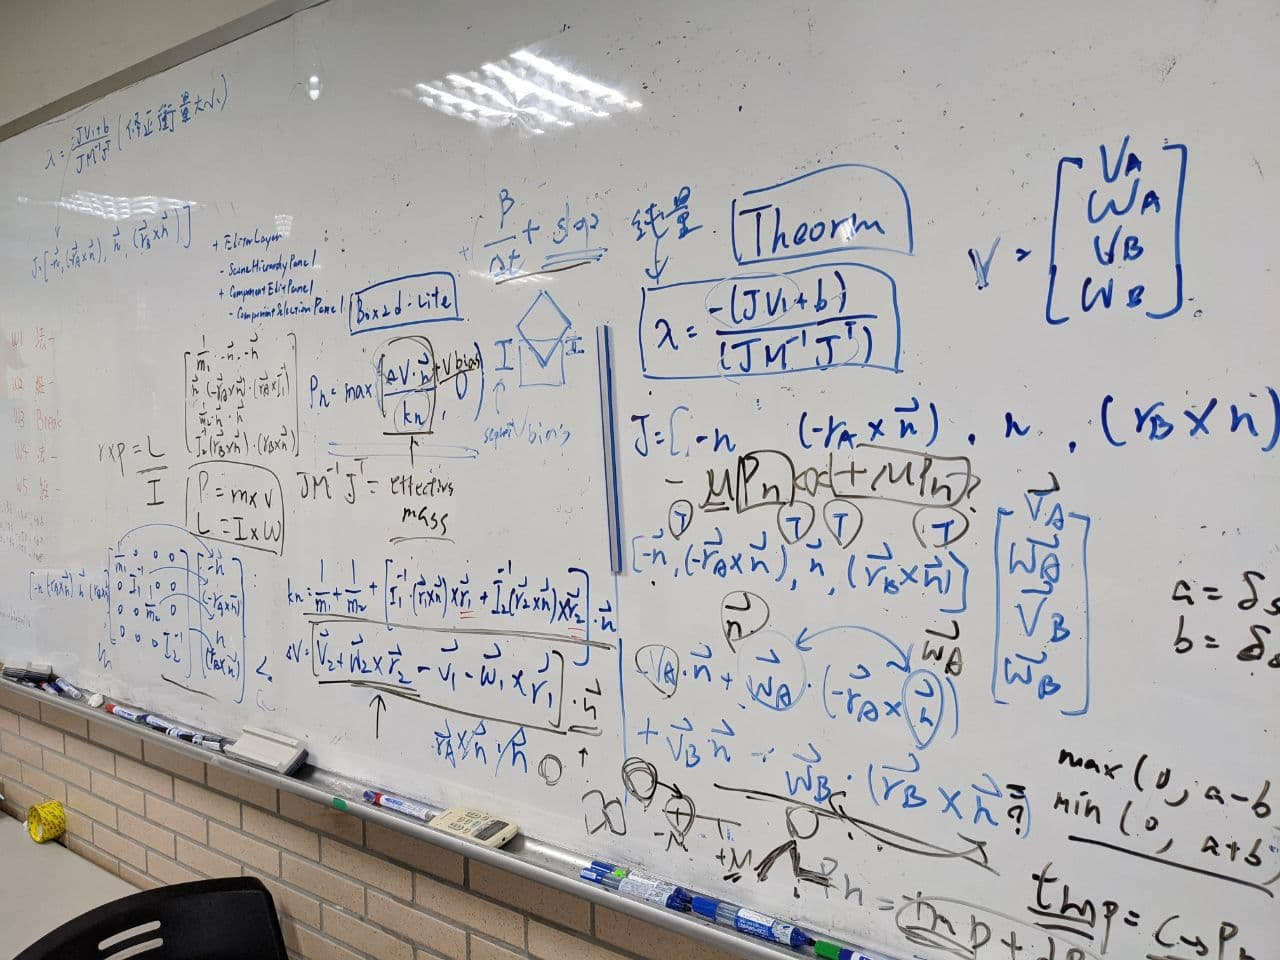
\includegraphics[width=0.8\textwidth]{./resources/ch6/halloworld_1.jpg}
    \end{center}
\caption*{被我寫滿物理證明的實驗室白板}
% \label{fig:ch6_whiteboard}
\end{figure}

除了與網路上無緣無故交到的筆友和議程上的講者,我也透過講者的關係下,拿到遊戲物理界大老的系列教學影片。那短短兩三個小時幾部的影片讓我真正了解到比較深層的理論。
如果以程式語言的學習歷程來比喻,在前期自己看程式以及與網路筆友的討論,像是學習高階語言一樣,大概能知道淺層的物理原理,但是再透過那系列的教學影片之後,又知道了有些東西的係數是這樣推倒而來,
就如同學習到組合語言一樣,能跟精確地知道整個程式運作的來龍去脈。除此之外,我也試著自己證明遊戲物理引擎的物理參數,看看真的是不是如程式寫得一樣,並自己在試著實作一次。
此外,覺得我自己還想更精進的部分,是希望以後能夠自己實作出3D的遊戲引擎,以及實作空氣阻力、彈簧...等更精細的物理模擬。

實作的過程中,很常被C++的語法及語言特性坑殺。舉個最經典的例子,最常遇到的應該就是循環引入的問題,編譯器卻沒告訴你哪裡出了問題,導致我花了很多時間來找bug。
我自認為我在實作遊戲物理邏輯中的部分,跟解決C++錯誤所花的時間比起來,修C++ BUG的時間真的佔了我大部分的時間。不過也從中學習到很多技巧。這些東西可能是課堂學不到的,
大部分都得靠網路或是同學之間討論,才能夠把這些複雜又惱人的 BUG 解掉。此外,在整個專案當中,隨著時間增長的程式碼,漸漸地讓編譯速度變得相當緩慢,裡面的 Warning 也越來越多,
這也是我很頭痛的部分。到專案後期,常常花的時間都不是在改程式碼,而是在等編譯。包括我現在寫心得的此時此刻,都是在等待的期間撰寫出來的。

另外,與團隊的交流也很重要,過程中有相當多的磨合以及很多的取捨,不過目的其實都是為了整個專案更好。比較愧疚的部分,是這次沒有參與到遊戲引擎整個開發的部分,
引擎內部裡面的細節我沒有仔細的接觸過。主要因為光花那些時間證明物理以及實作就踩了許多坑也耗費了很多時間和冤枉路,加上我自己的資質駑鈍和我的英文能力,
以及,真正研究過遊戲物理的人真的很少,資源也相對地難找,也就導致我沒有參與到整個引擎最主要的開發部分。最後,我想感謝我的組員們,雖然引擎不是最完美的,
但我相信從開發過程應該都學到不少的東西以及經驗,也很感謝實驗室的學長和同學,陪我們度過一次又一次的Bug。

\begin{center}

\includegraphics[height=9cm]{./resources/rish_2.png}
\end{center}

\newpage